\documentclass[16pt, aspectratio=43,compress]{beamer}

% Add paths to look through
\makeatletter
\def\input@path{{Classes/}{preface/}{introduction/}{method/}{structure/}{dynamics/}{crystallisation/}{conclusion/}{appendix/}}
\makeatother

\mode<presentation>
{
  \usetheme{Ilmenau}
  %\setbeamercovered{transparent}
  \useoutertheme{myframes}
}

%\usefonttheme[onlymath]{sansserif}

\usepackage{common}
\usepackage{tikz}
\usepackage{textpos}
\usepackage{multimedia}
\usepackage{media9}
\usepackage{pgfpages}
\usepackage[cm]{sfmath}
%\usepackage{achemso}
\usepackage{animate}

\usepackage{biblatex}
\bibliography{crystal.bib}

\graphicspath{{preface/figures/}{method/figures/}{introduction/figures/}{dynamics/figures/}{structure/figures/}{crystallisation/figures/}{presentation/}}
\renewcommand{\footcite}{\footfullcite}

\setbeamertemplate{navigation symbols}{}

\renewcommand{\footnoterule}{}
%\renewcommand{\footnotemark}{}
\renewcommand*{\footnotesize}{\fontsize{5}{7}}

\makeatletter
\def\@listi{\leftmargin\leftmargini
              \topsep    2ex
              \parsep    0\p@   \@plus\p@
              \itemsep   4ex}
\makeatother

\newcommand*{\myhat}[1]{\skew{3}{\hat}{#1}}

\title[Shapes on a Plane]{The Role of Molecular Shape on the Properties of the Condensed Phase:\\ A Simulation Study}
\author{Malcolm Ramsay}


\usecolortheme{whale}
\usefonttheme{professionalfonts}

%\setbeameroption{show notes on second screen}

\setbeamerfont{frametitle}{size={\fontsize{22}{24}}}


\begin{document}

%%%%%%%%%%%%%%%%%%%%%%%%%%%%%%%%%%%%%%%%%%%%%%%%

\begin{frame}
  \titlepage
\end{frame}


%%%%%%%%%%%%%%%%%%%%%%%%%%%%%%%%%%%%%%%%%%%%%%%

\begin{frame}{Outline}
    \tableofcontents
\end{frame}


%%%%%%%%%%%%%%%%%%%%%%%%%%%%%%%%%%%%%%%%%%%%%%%

\section{Background}
\subsection{Molecular Crystals}

\begin{frame}{Unit Cells}
    \begin{columns}
        \begin{column}{0.5\linewidth}
            \begin{itemize}
                \item The building blocks of crystals
                \item Can be used to tile all of space
            \end{itemize}
        \end{column}
        \begin{column}{0.5\linewidth}
            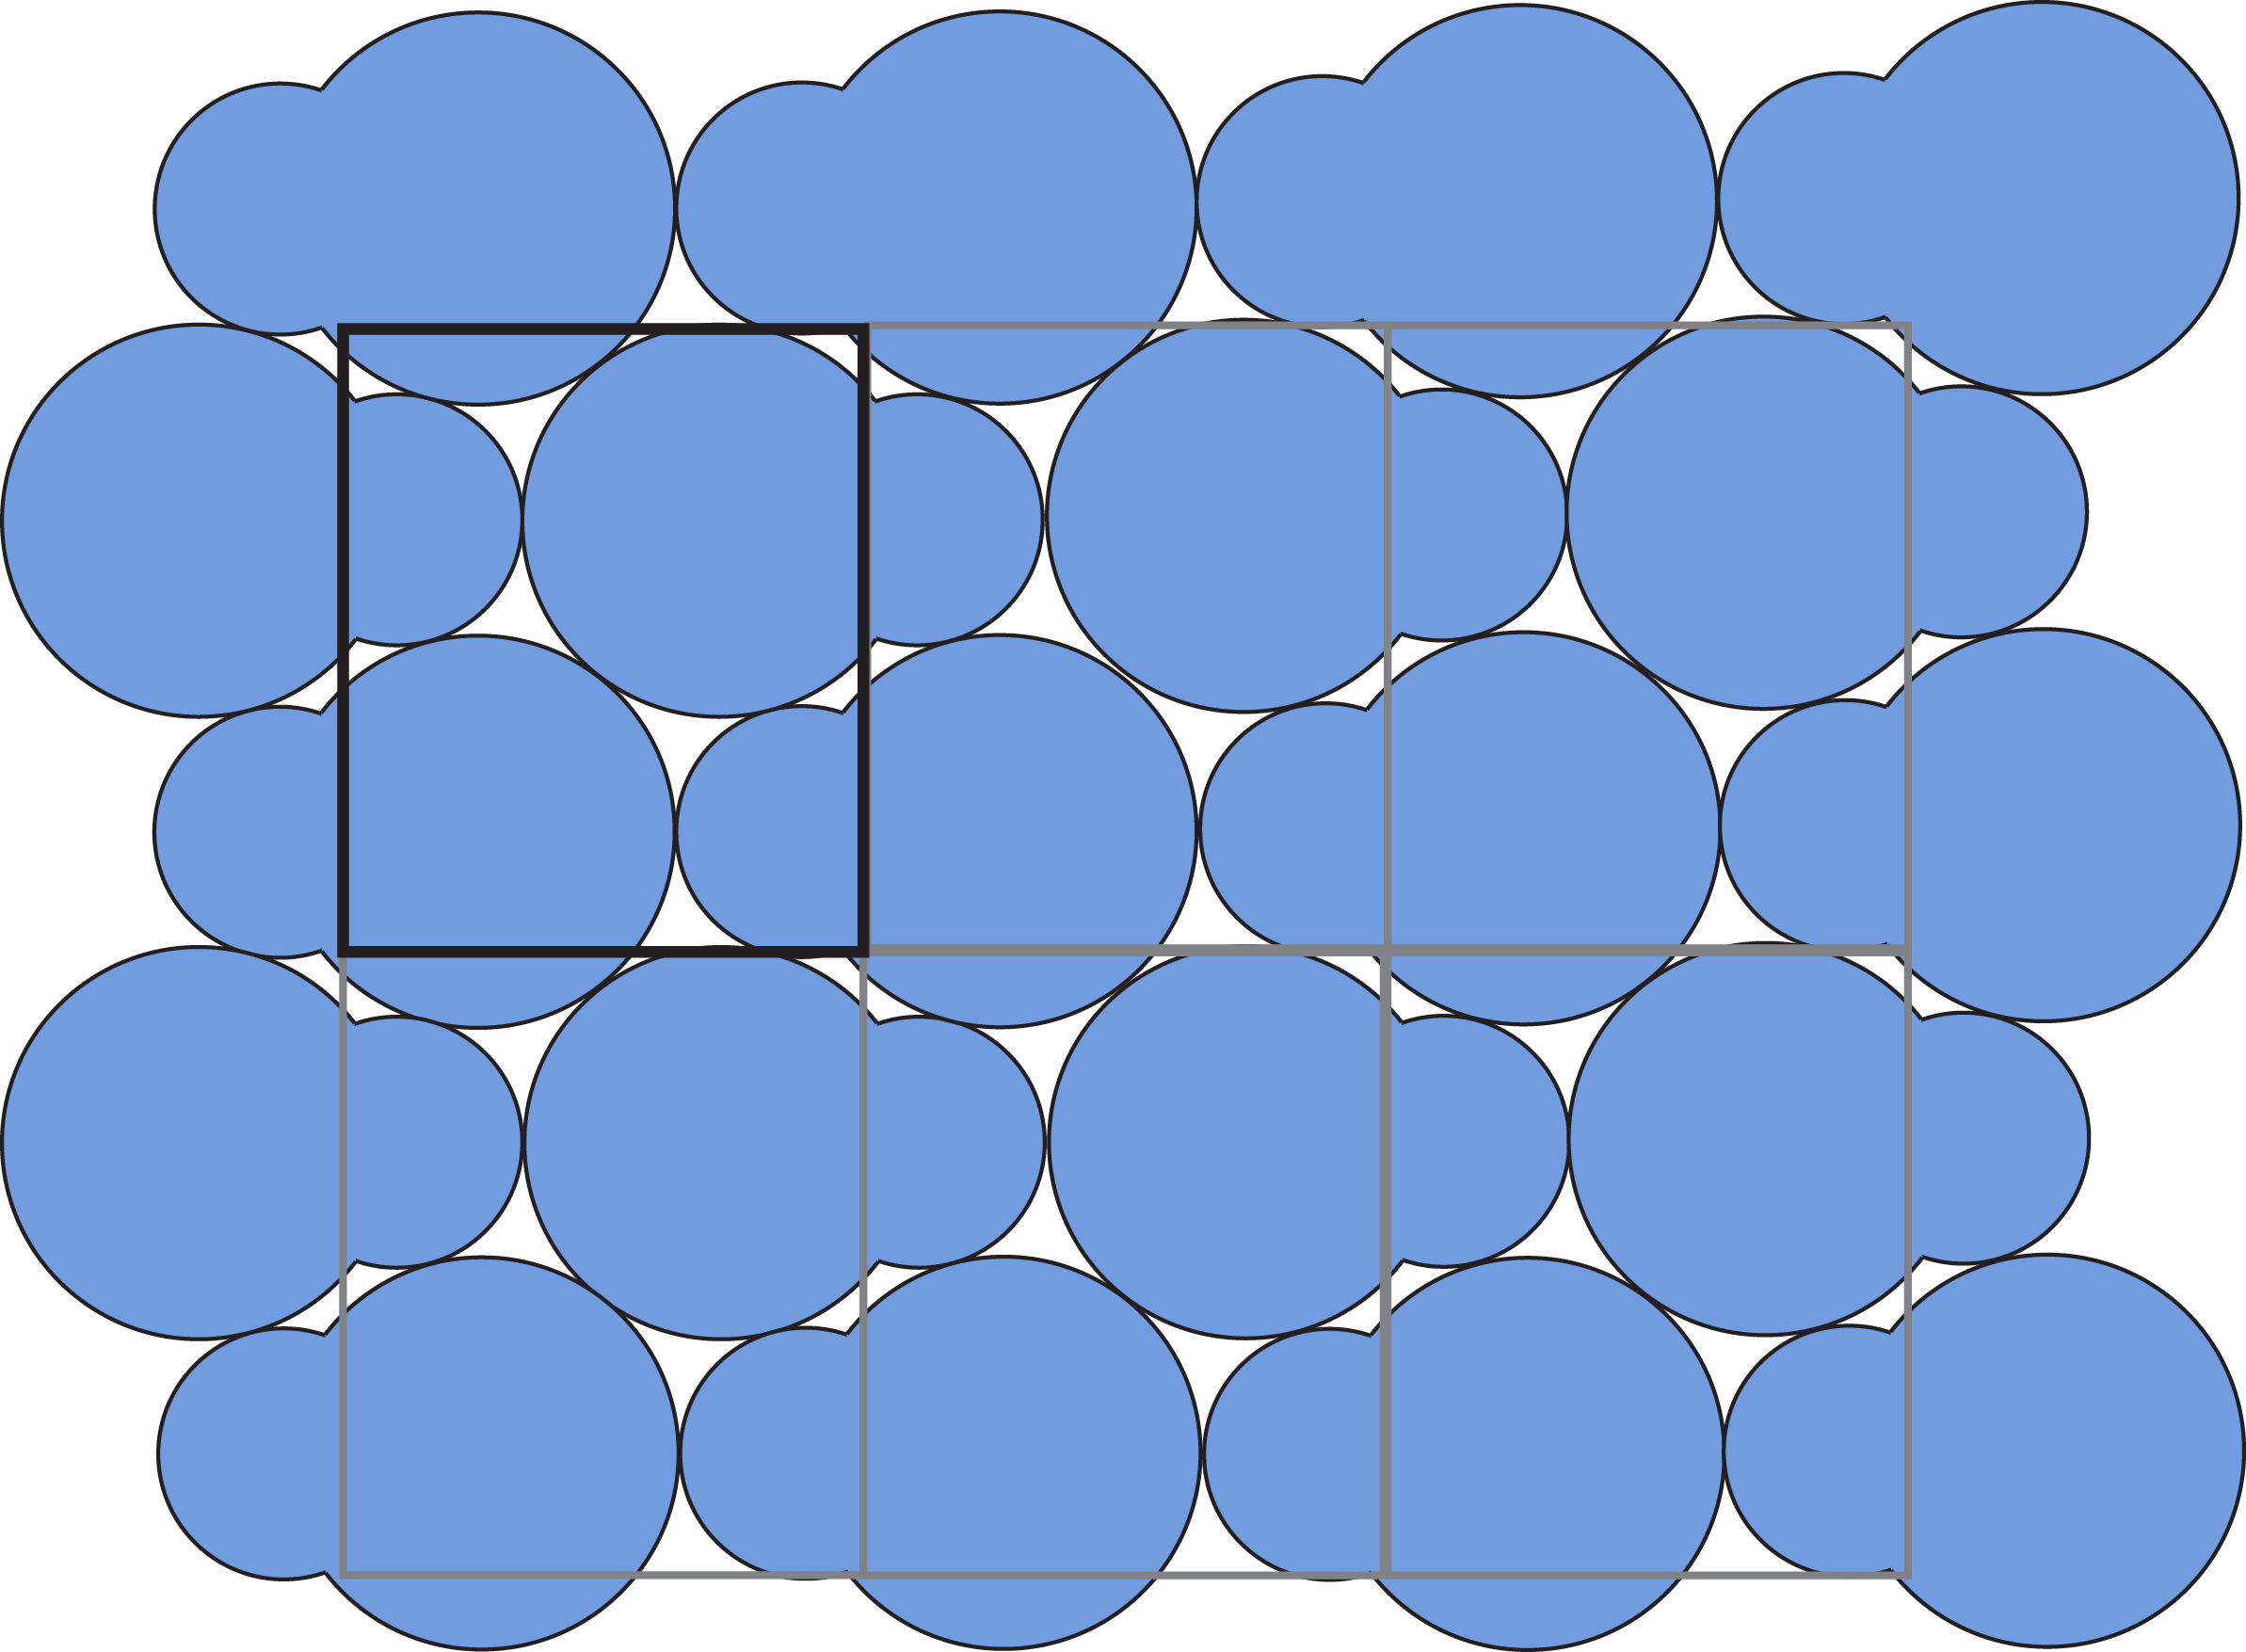
\includegraphics[width=\textwidth]{unit_cell}
        \end{column}
    \end{columns}
\end{frame}

%%%%%%%%%%%%%%%%%%%%%%%%%%%%%%%%%%%%%%%%%%%%%%%

\begin{frame}{Wallpaper Groups}
    \begin{columns}
        \begin{column}{0.5\linewidth}
            \begin{itemize}
                \item Give us the symmetry elements
                \item Minimal representation of the unit cell
            \end{itemize}
        \end{column}
        \begin{column}{0.5\linewidth}
            \centering
            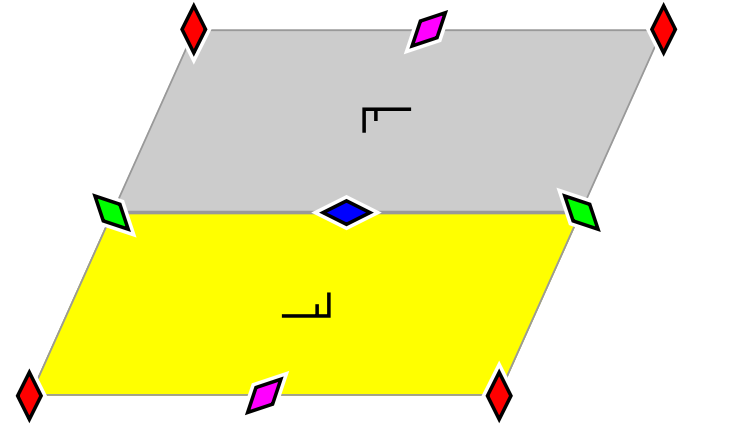
\includegraphics[width=\textwidth]{p2}\\
            p2\\
            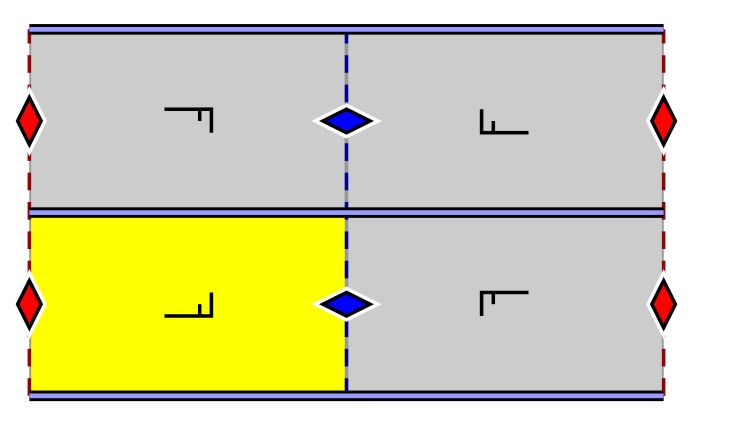
\includegraphics[width=\textwidth]{p2mg}\\
            p2mg
        \end{column}
    \end{columns}
\end{frame}

%%%%%%%%%%%%%%%%%%%%%%%%%%%%%%%%%%%%%%%%%%%%%%%

\subsection{Molecular Liquids}

\begin{frame}{Dynamic Quantities}
    \begin{itemize}
        \item MSD
        \item Diffusion Constant
        \item Rotational Relaxation
        \item Relaxation time
        \item Debye Waller term
    \end{itemize}
\end{frame}

\begin{frame}{Supercooled Liquids}
    \begin{columns}
        \begin{column}{0.5\linewidth}
            \begin{itemize}
                \item Liquid below the freezing point
                \item An integral part of crystallisation
                \item Temperatures at which nucleation becomes stable
            \end{itemize}
        \end{column}
        \begin{column}{0.5\linewidth}
            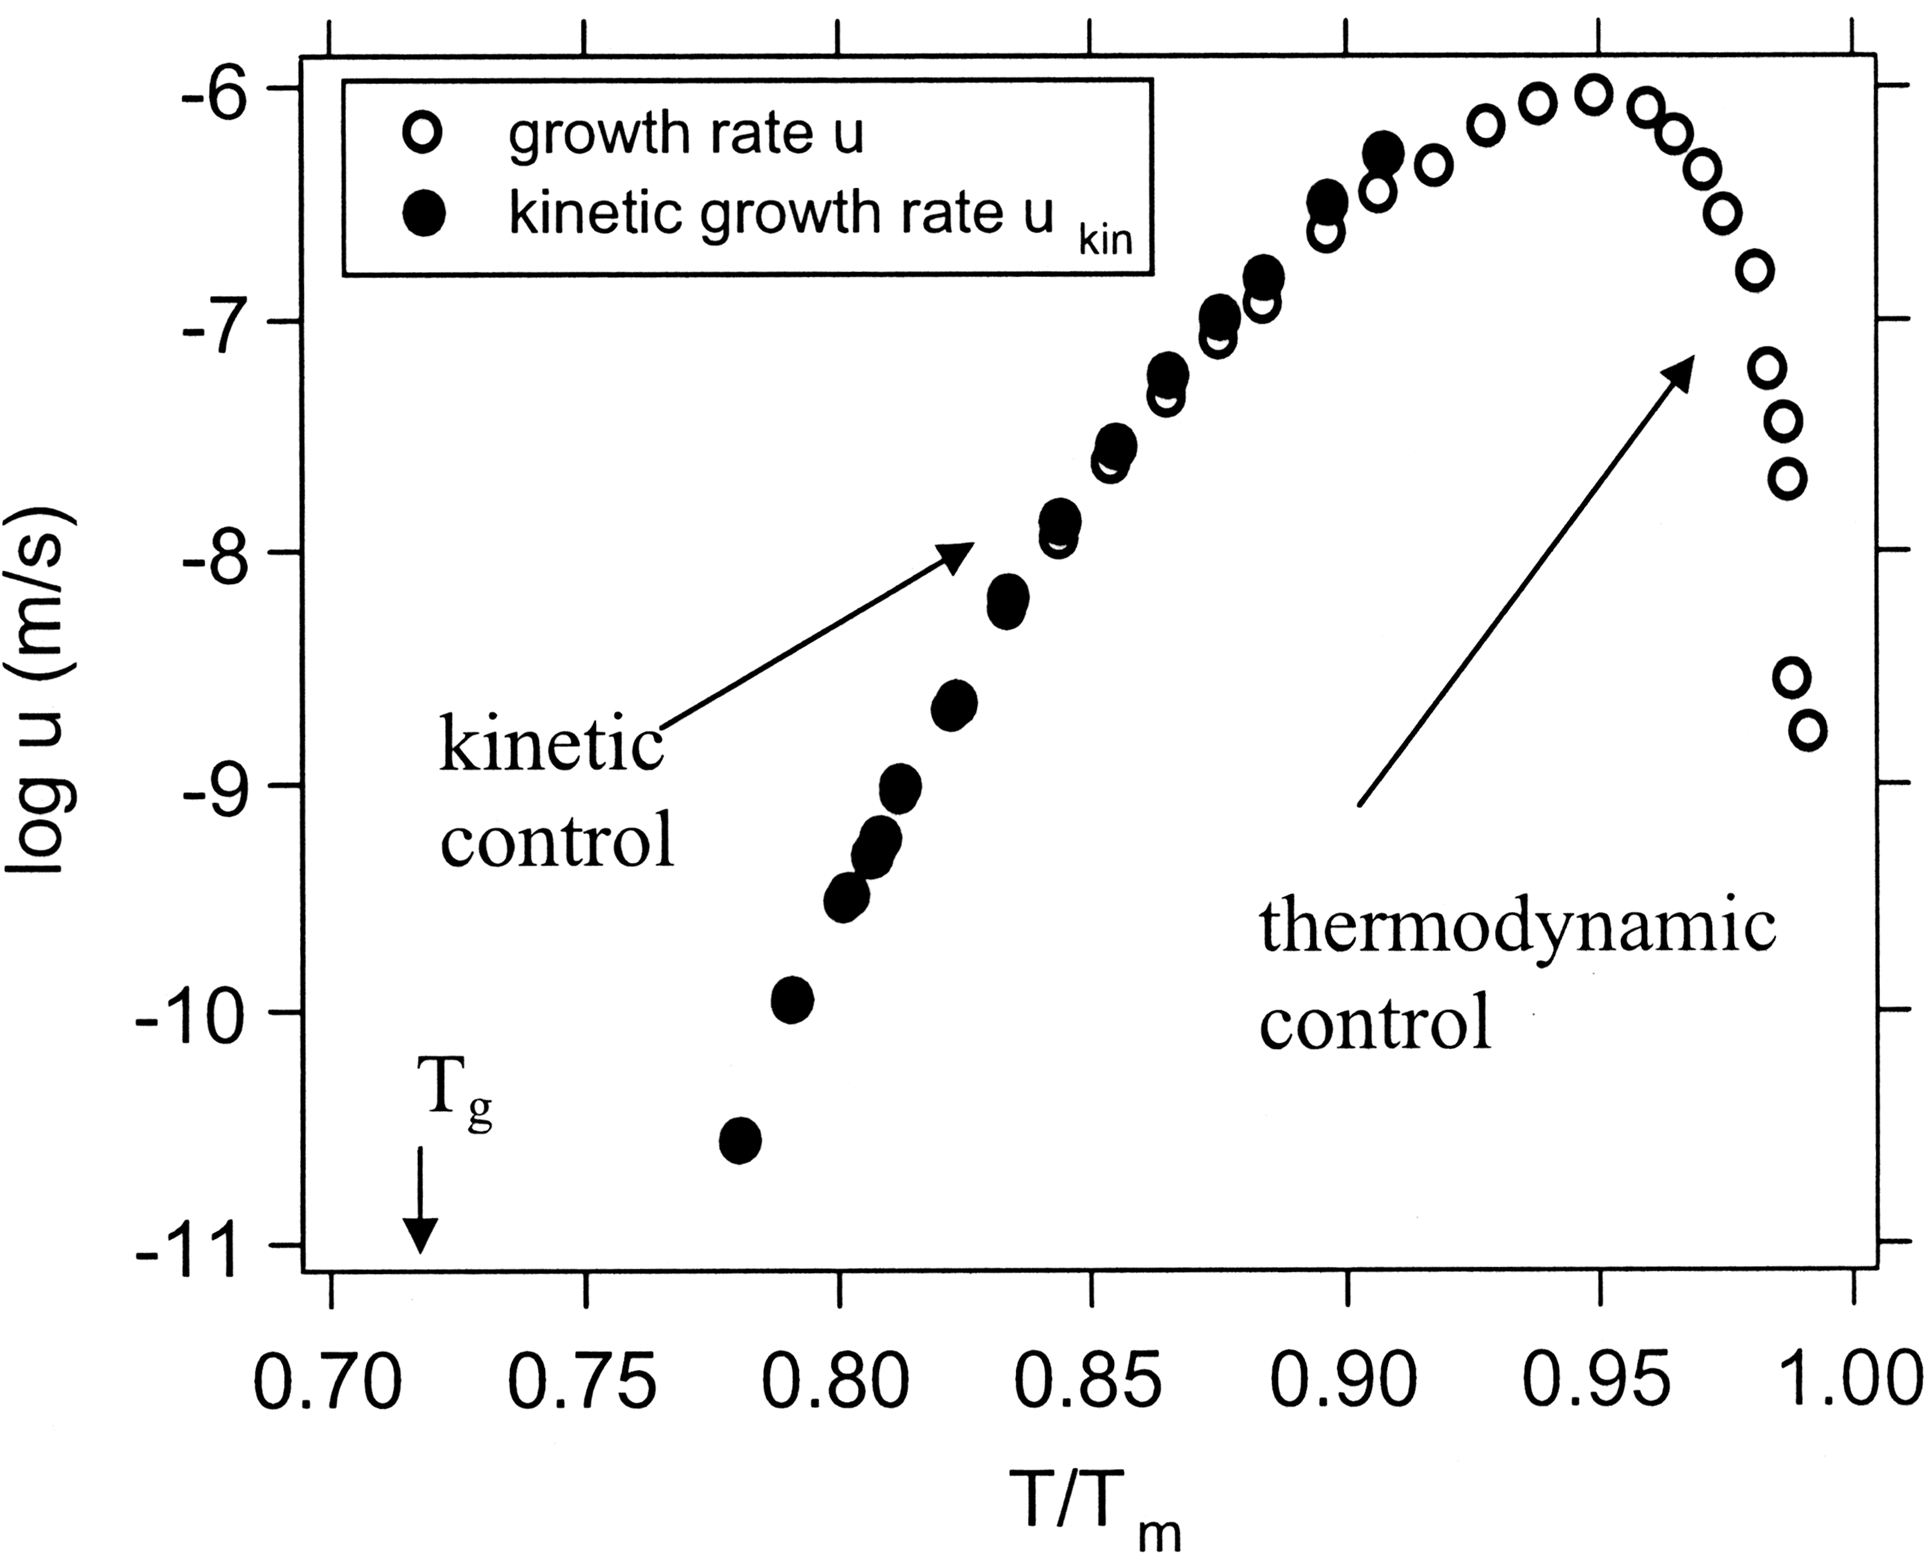
\includegraphics[width=\textwidth]{crystal-growth}
        \end{column}
    \end{columns}
\end{frame}

\begin{frame}{Liquid Fragility}
    \begin{columns}
        \begin{column}{0.5\linewidth}
            \begin{itemize}
                \item Description of liquid behaviour close to glass transition
                \item Silica (\ce{SiO2}) a strong liquid shows linear behaviour
                \item {\em o}-Terphenyl a weak liquid large deviation from linear
            \end{itemize}
        \end{column}
        \begin{column}{0.5\linewidth}
            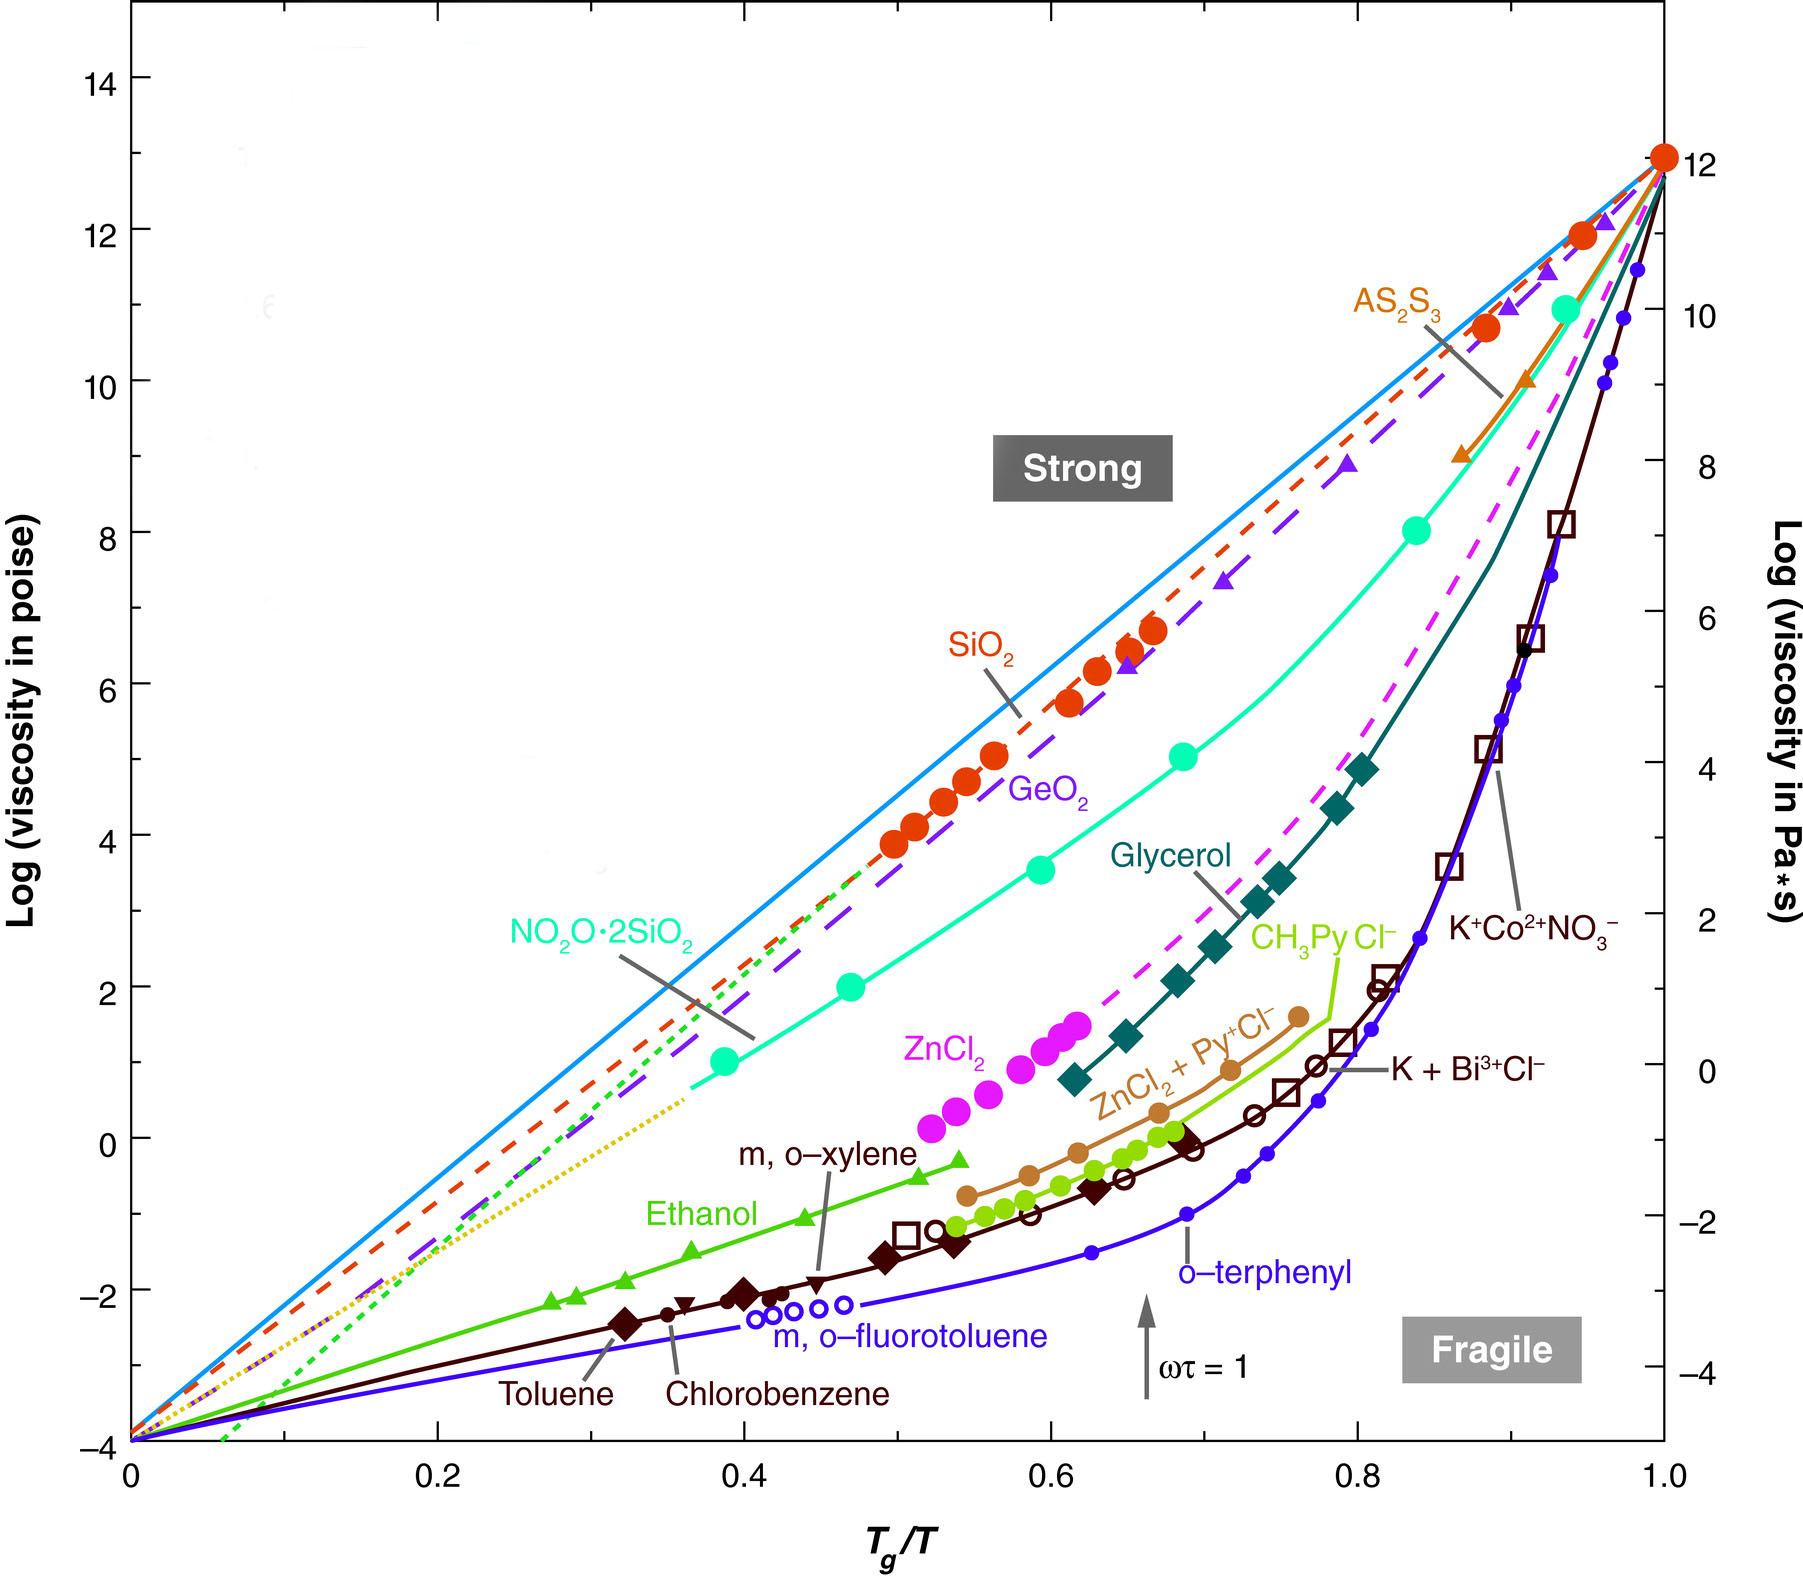
\includegraphics[width=\textwidth]{angell}
        \end{column}
    \end{columns}
\end{frame}

\section{Dynamics}

\subsection{Molecules}

\begin{frame}{Molecules chosen to Study}
    \begin{columns}
        \begin{column}{0.5\linewidth}
            \centering
            \includegraphics[width=\textwidth]{sone}\\
            \done
        \end{column}
        \begin{column}{0.5\linewidth}
            \centering
            \includegraphics[width=\textwidth]{tri}\\
            \tri
        \end{column}
    \end{columns}
\end{frame}

\subsection{Defining Dynamic Quantities}

\begin{frame}{Mean Squared Displacement}
    \begin{columns}
        \begin{column}{0.5\linewidth}
            \begin{itemize}
                \item Measure of the motion of the centers of mass
            \end{itemize}
            \begin{align*}
                 MSD(t) &= \langle \Delta \vect{r}(t)^2 \rangle,\\
                 \Delta \vect r(t) &= \sqrt{(x(t) - x_0)^2 + (y(t) - y_0)^2}
            \end{align*}
        \end{column}
        \begin{column}{0.5\linewidth}
            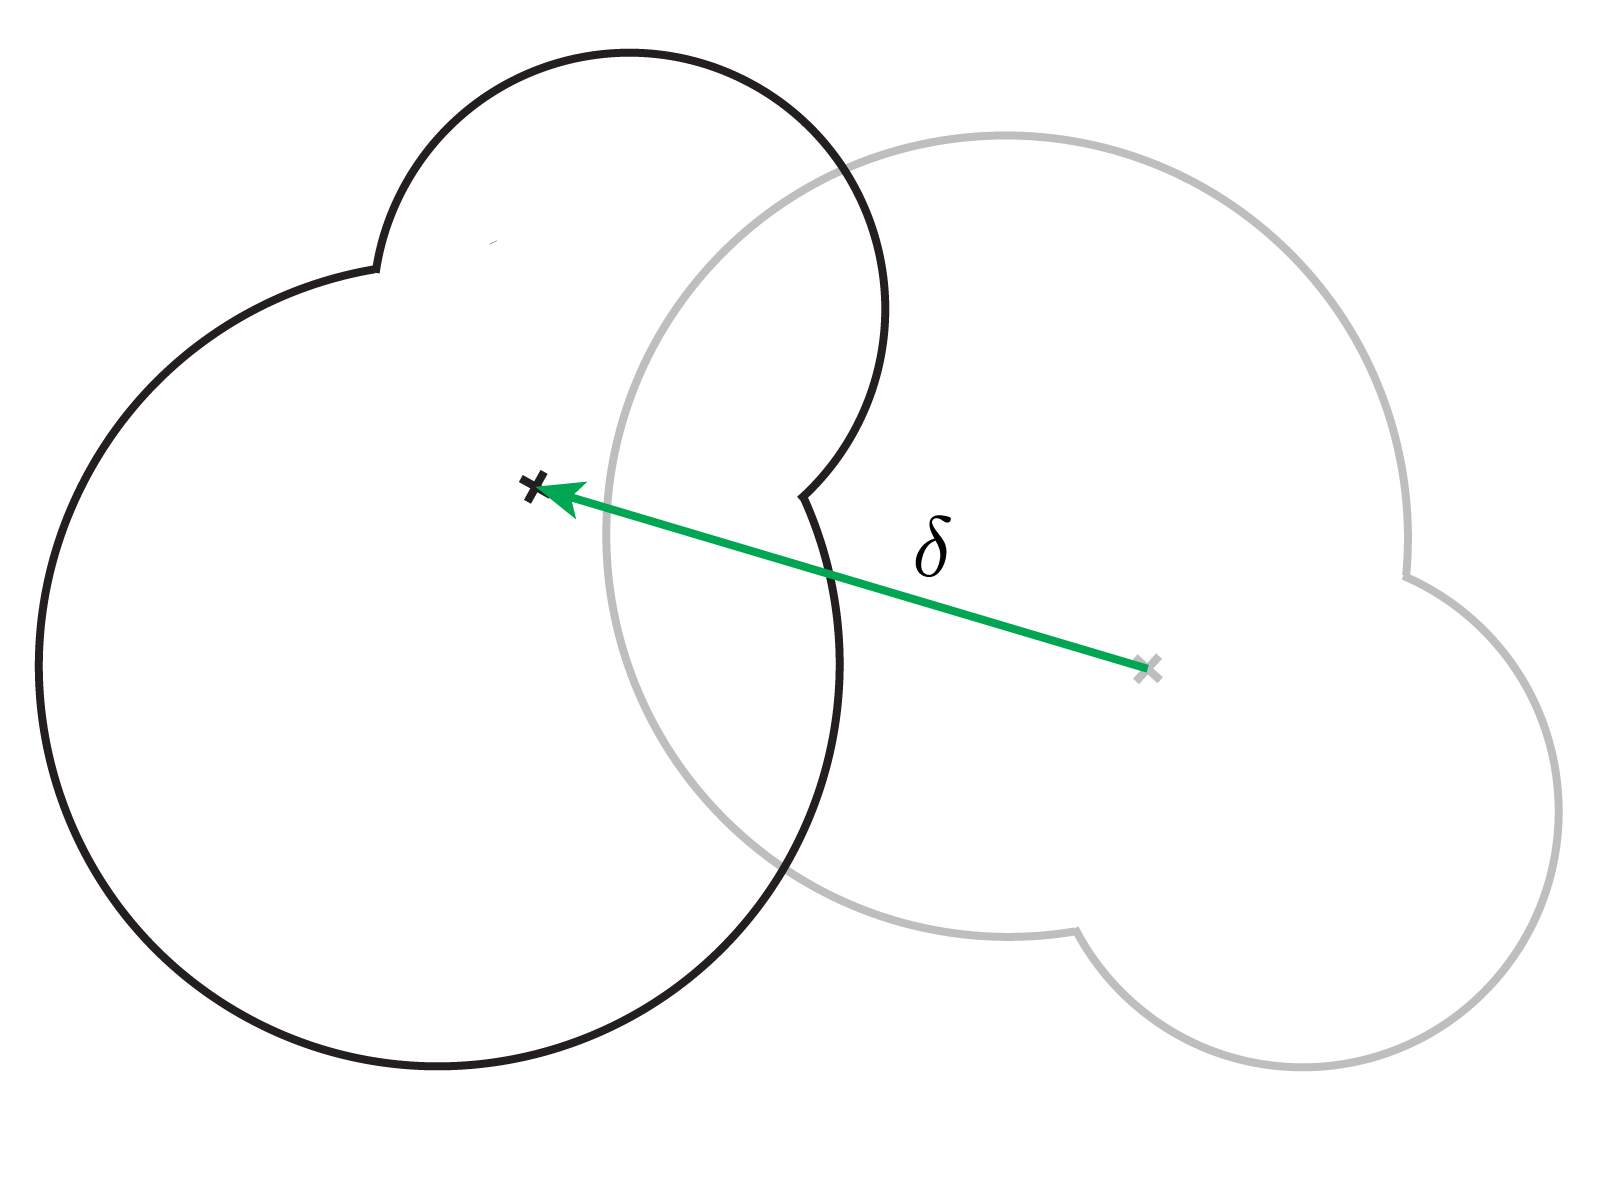
\includegraphics[width=\textwidth]{msd}
        \end{column}
    \end{columns}
\end{frame}

\begin{frame}{Rotational Relaxation}
    \begin{columns}
        \begin{column}{0.5\linewidth}
            \begin{itemize}
                \item Measure of the rotational motion
            \end{itemize}
            \begin{align*}
                C_n(t) &= \langle \vect{e}(0) \cdot \vect{e}(t) \rangle
            \end{align*}
        \end{column}
        \begin{column}{0.5\linewidth}
            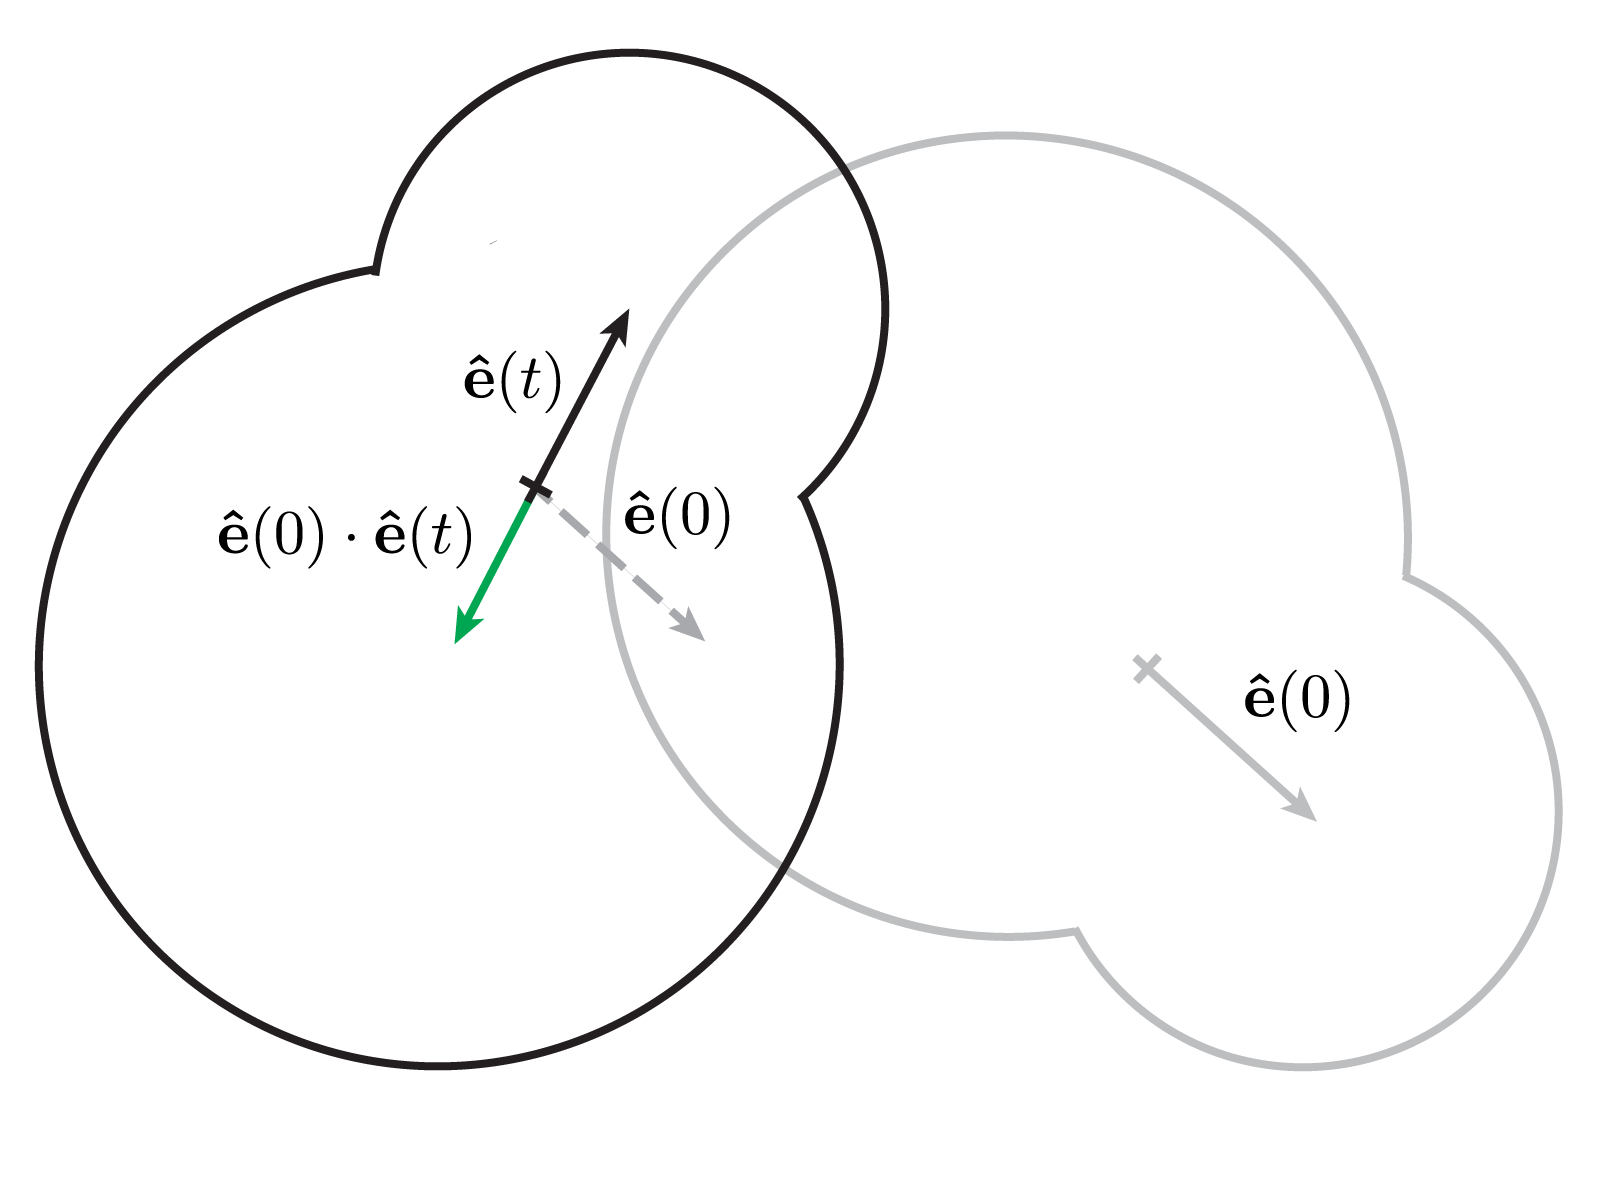
\includegraphics[width=\textwidth]{rot}
        \end{column}
    \end{columns}
\end{frame}

\begin{frame}{Structural Relaxation}
    \begin{columns}
        \begin{column}{0.5\linewidth}
            \begin{itemize}
                \item Measure of the relaxation of the structure
            \end{itemize}
            \begin{align*}
                  F(t) = \left \langle \begin{cases}
                        \quad0 &\text{if } \Delta \vect r > 0.3 \\
                        \quad1 &\text{if } \Delta \vect r \leq 0.3
                  \end{cases} \quad \right \rangle
            \end{align*}
        \end{column}
        \begin{column}{0.5\linewidth}
            \centering
            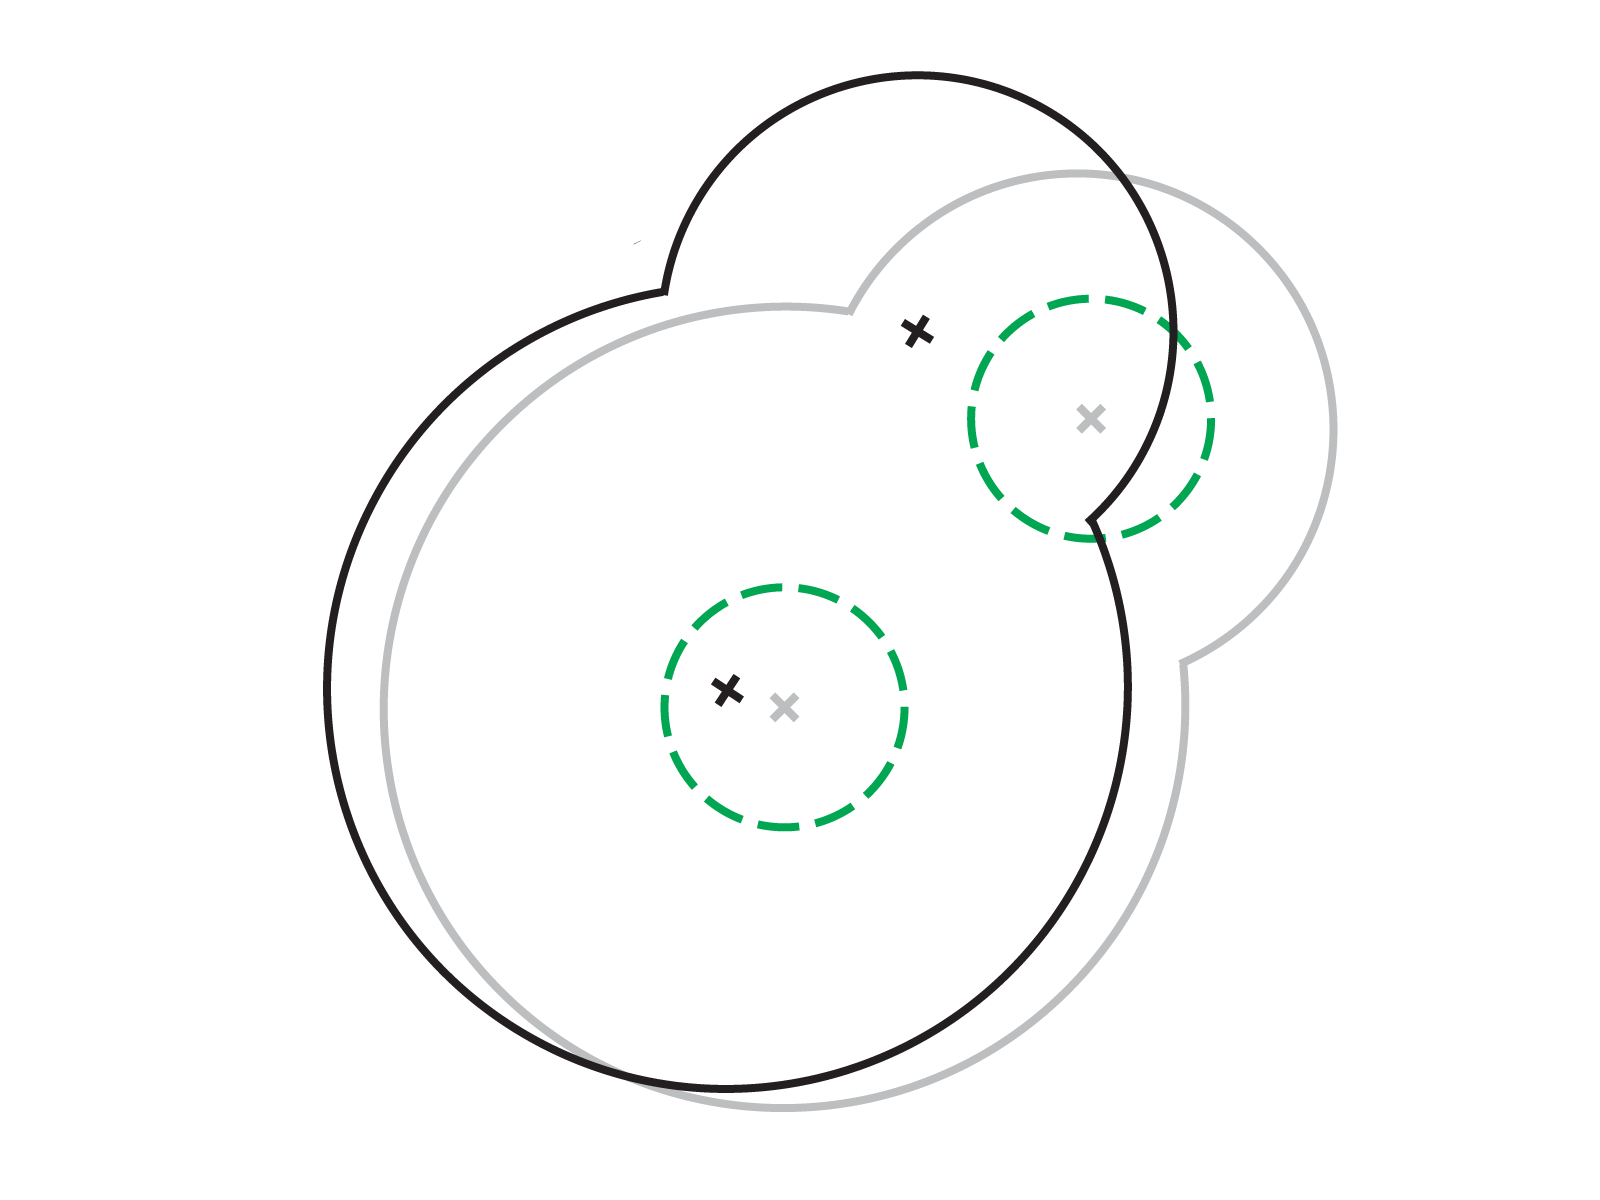
\includegraphics[width=0.8\textwidth]{struct}
        \end{column}
    \end{columns}
\end{frame}

\subsection{Dynamic Quantities}

\begin{frame}{Diffusion Constant}
    \centering
    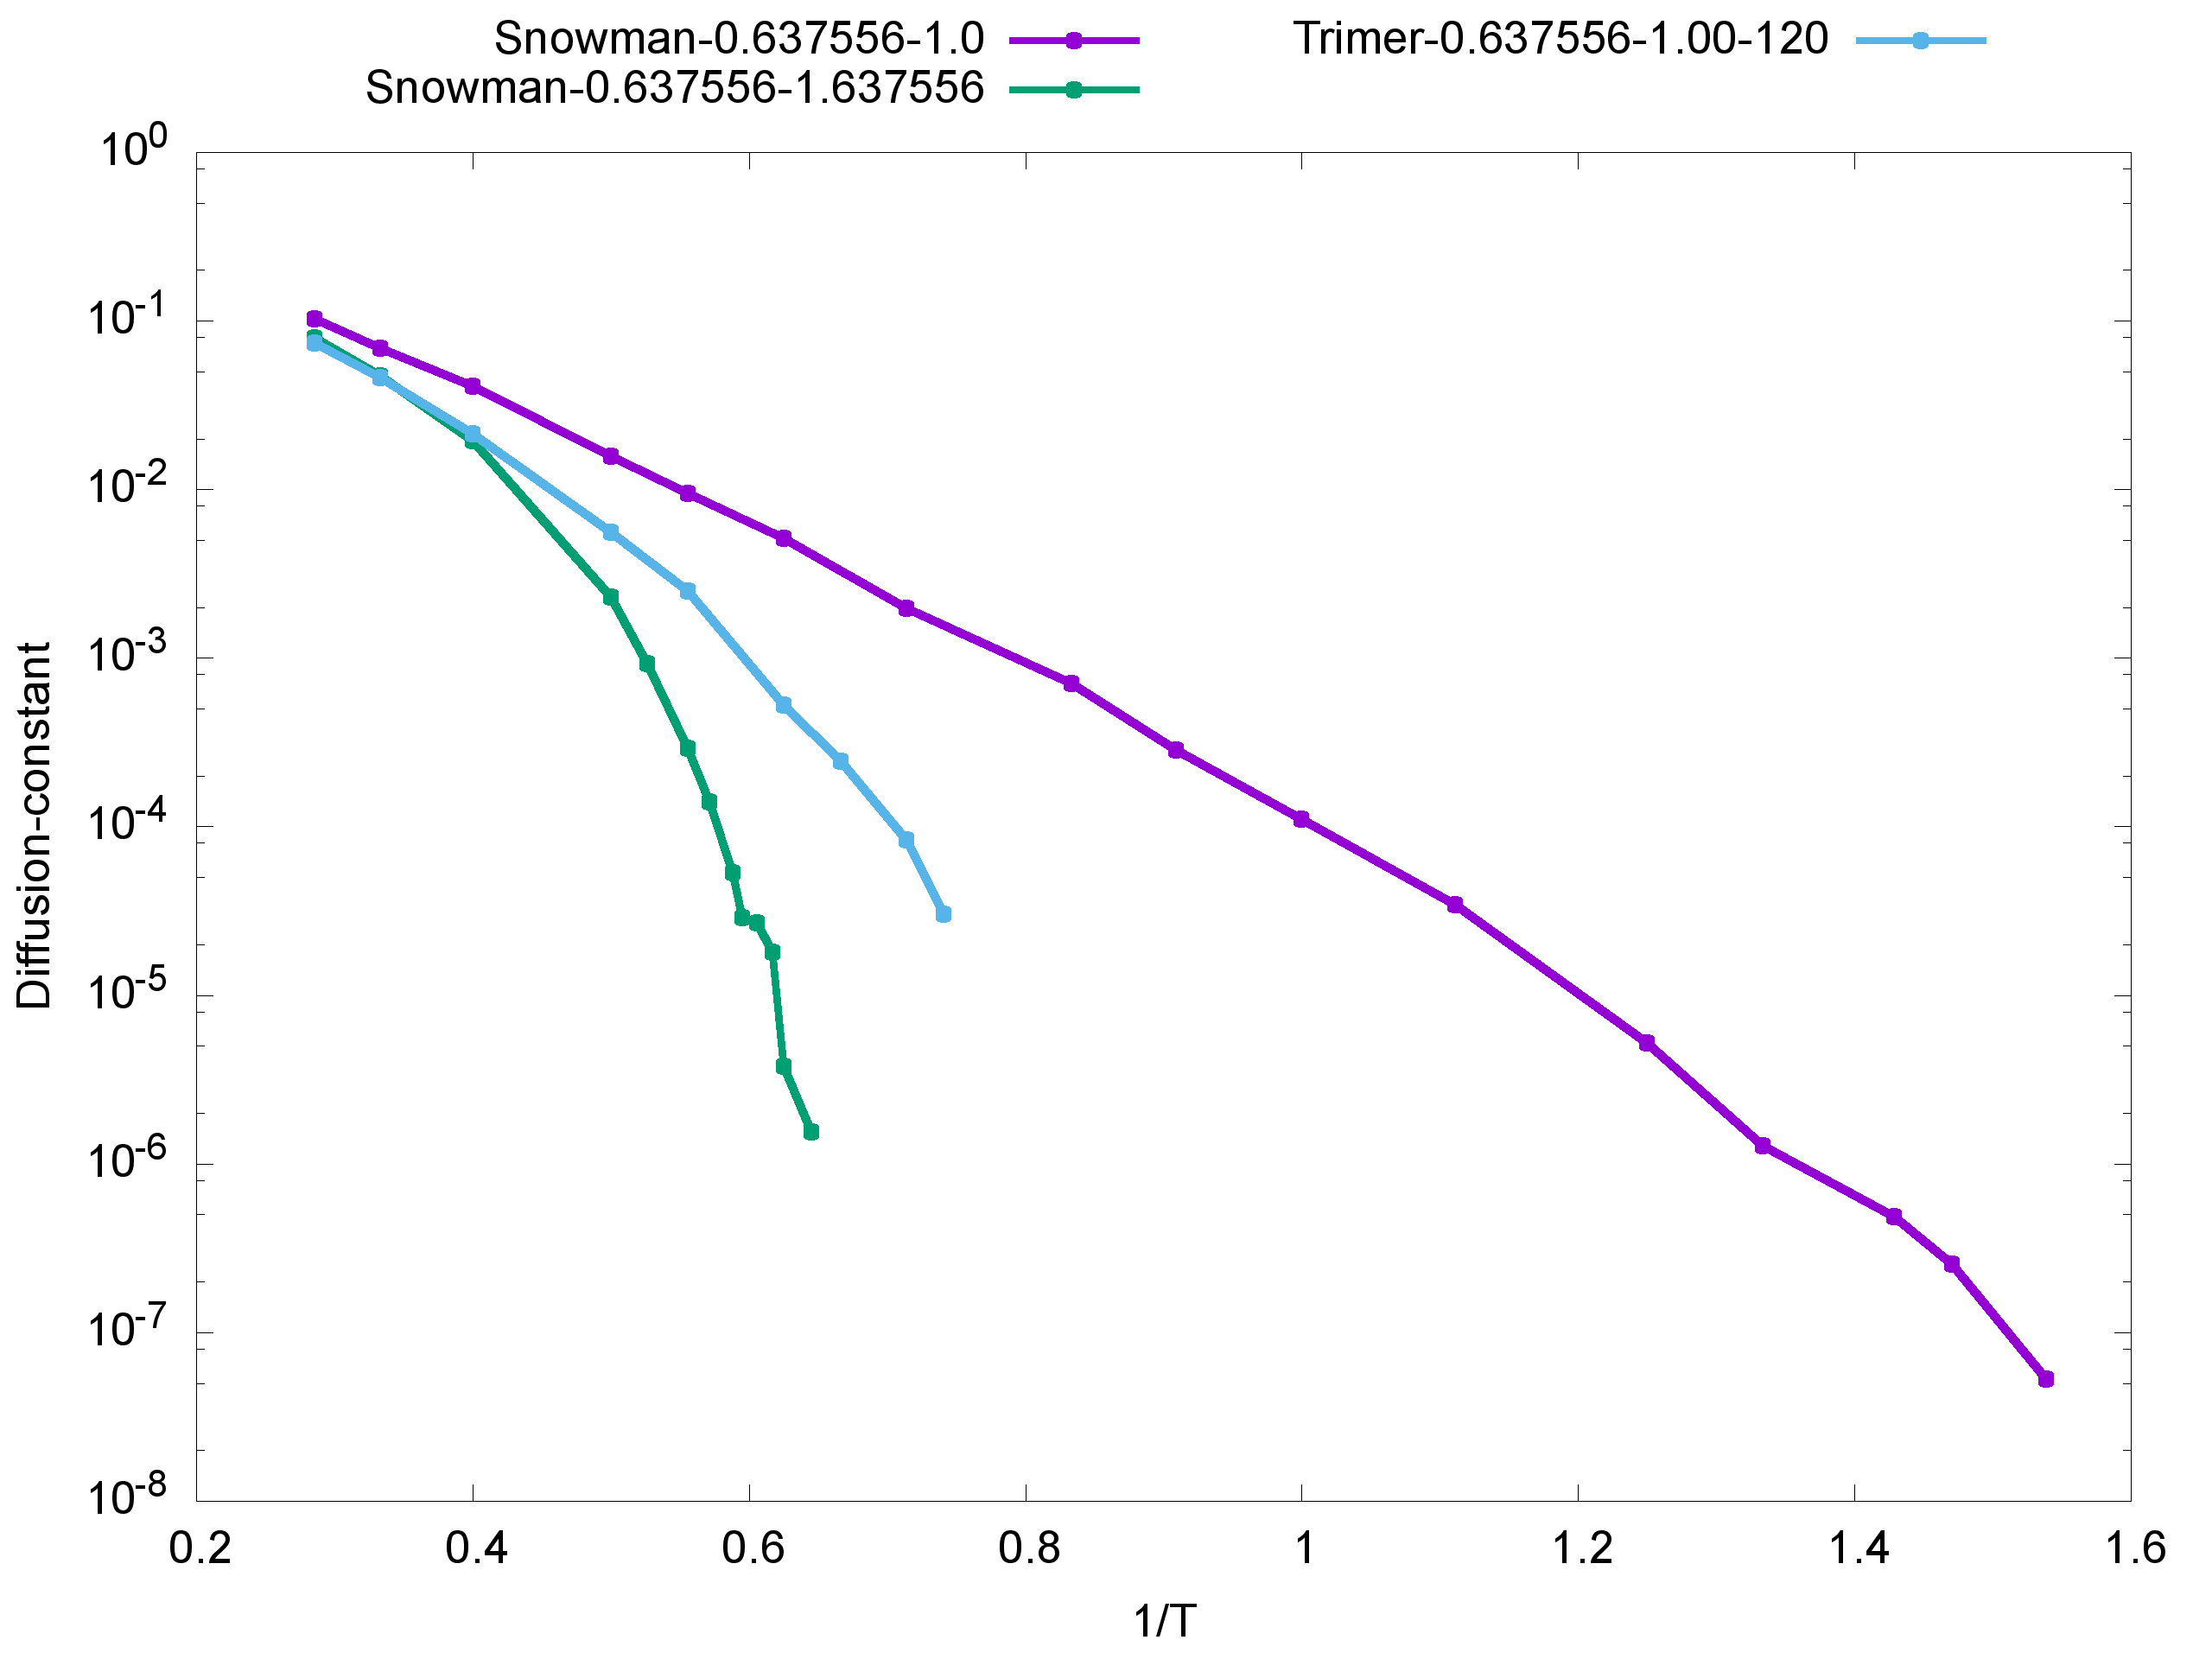
\includegraphics[width=\textwidth]{Diffusion-constant}
\end{frame}

\begin{frame}{Rotational Relaxation}
    \centering
    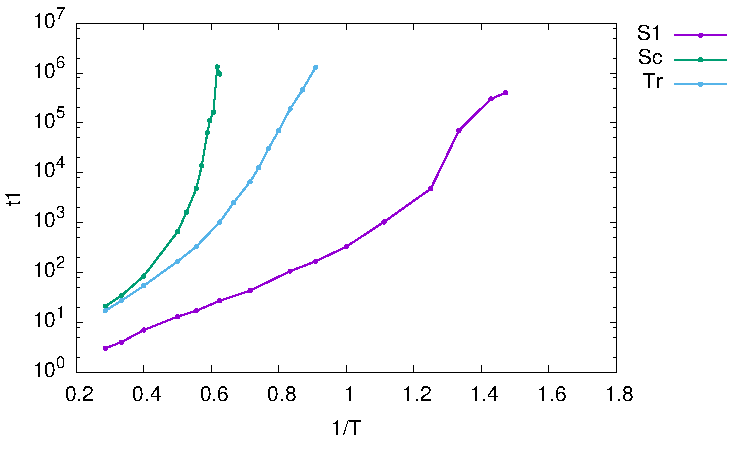
\includegraphics[width=\textwidth]{t1}
\end{frame}

\begin{frame}{Structural Relaxation}
    \centering
    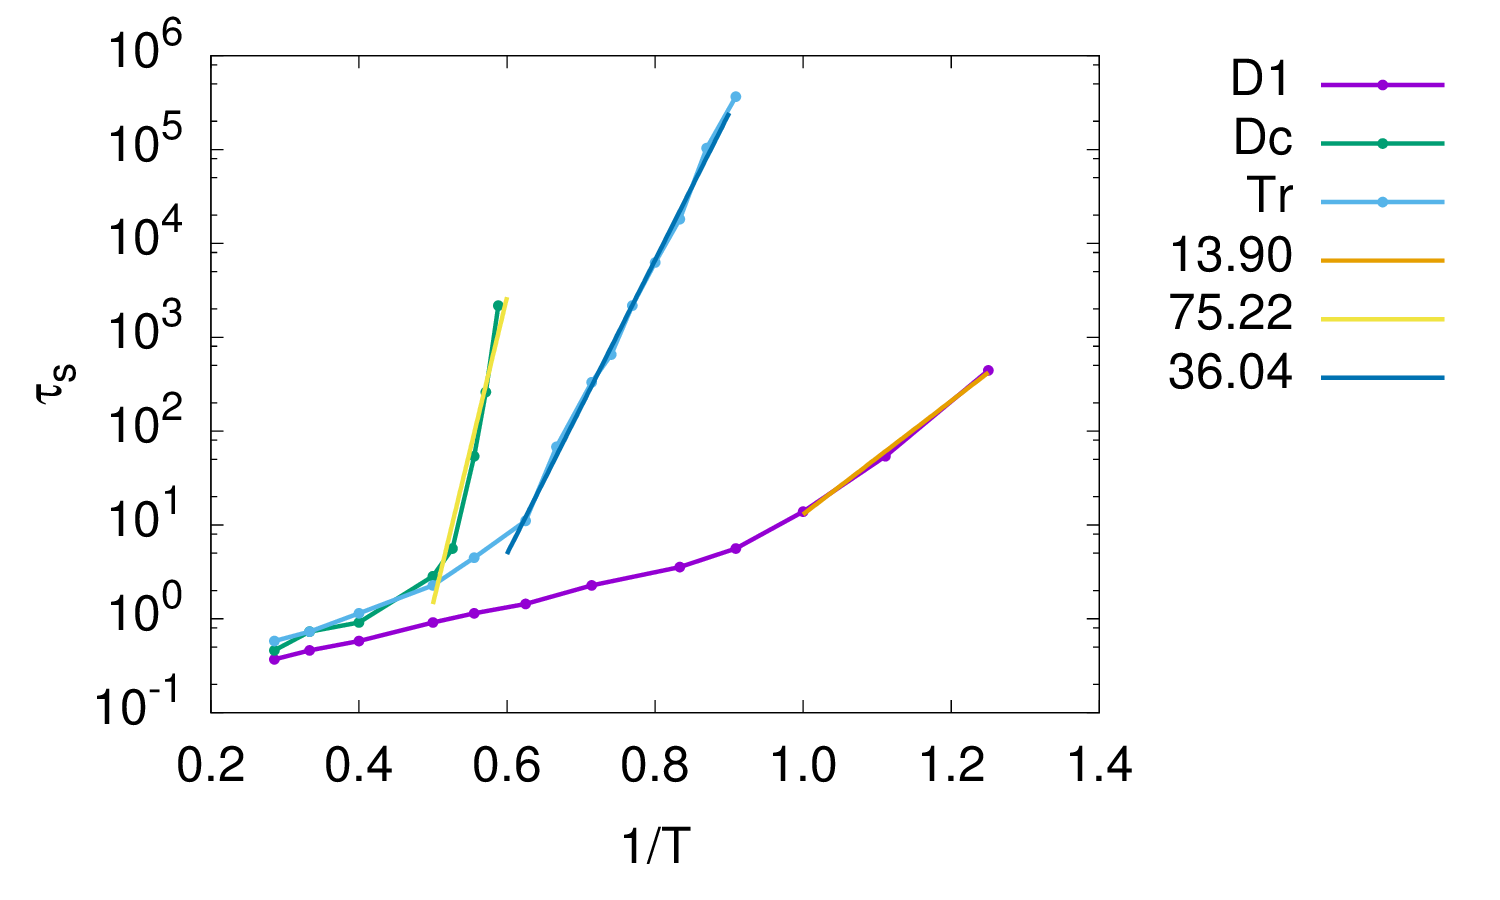
\includegraphics[width=\textwidth]{ts}
\end{frame}

\begin{frame}{Short Range Diffusion}
    \centering
    \includegraphics[width=\textwidth]{{{DW.D}}}
\end{frame}

\begin{frame}{Dynamic Inhomogeneities}
    \centering
    \includegraphics[width=\textwidth]{{{Trimer-1.15-0.637556-1.00-120-moved}}}
\end{frame}

\section{Crystallisation}

\subsection{Crystal Structure}

\begin{frame}{Stable Crystals}
\end{frame}

\begin{frame}{Identifying the Crystal Phase}
\end{frame}

\subsection{Crystal Dynamics}

\begin{frame}{Two Phase Systems}
\end{frame}


\begin{frame}{Nucleation}
    \vspace{-3pt}
    \animategraphics[width=\linewidth]{12}{presentation/movie/}{0001}{0333}
\end{frame}

\section{Conclusion}

\begin{frame}{Future Work}
\end{frame}


\begin{frame}{Acknowledgements}
\end{frame}

\subsection{Questions}

\begin{frame}{Questions}
\end{frame}

\end{document}


